\chapter{Bottom-Up Parsing}
\label{cha:BottomUp}

The natural counterpart to top-down parsing is bottom-up parsing, where trees are built starting at the leaves and moving towards the root.
Like top-down parsing, bottom-up parsing is fairly simple and builds the foundation of a variety of parsing algorithms.
But just like top-down parsing, it has certain shortcomings regarding psycholinguistic adequacy.

\section{Intuition}
\label{sec:BottomUp_Intuition}
For illustration we use the same grammar as for the top-down parser in Lecture~\ref{cha:TopDown}.
%
\begin{center}
    \begin{tabular}{rrlp{3em}rrl}
        1)  & S   & \rewrite\ NP VP               &  & 
        6)  & Det & \rewrite\ a | the
        \\
        2)  & NP  & \rewrite\ PN                  &  & 
        7)  & N   & \rewrite\ car | truck | anvil
        \\
        3)  & NP  & \rewrite\ Det N               &  & 
        8)  & PN  & \rewrite\ Bugs | Daffy
        \\
        4)  & VP  & \rewrite\ Vi                  &  & 
        9)  & Vi  & \rewrite\ fell over
        \\
        5)  & VP  & \rewrite\ Vt NP               &  & 
        10) & Vt  & \rewrite\ hit
        \\
    \end{tabular}
\end{center}
%
A bottom-up parser essentially applies the rewrite rules in reverse.
If the current input $i$ appears on the right-hand side of a rewrite rule for $N$, replace $i$ by $N$.
%
\begin{center}
    \begin{tabular}{r|l}
        \textbf{string} & \textbf{rule}\\
        the & read input\\
        det & Det \rewrite the\\
        det anvil & read input\\
        det N & N \rewrite anvil\\
        NP & NP \rewrite Det N\\
        NP hit & read input\\
        NP Vt & Vt \rewrite hit\\
        NP Vt Daffy & read input\\
        NP Vt PN & PN \rewrite Daffy\\
        NP Vt NP & NP \rewrite PN\\
        NP VP & VP \rewrite Vt NP\\
        S & S \rewrite NP VP
    \end{tabular}
\end{center}

The order in which rules are applied once again gives rise to at least four different types of parsers, a helpful first approximation of which can be gleaned from the examples below.
The four trees below correspond to (in clockwise order) left-to-right depth first, right-to-left depth first, right-to-left breadth first, and left-to-right breadth first.
%
\begin{center}
    \begin{tikzpicture}
        \Tree
            [.\Lab{S}{12}{}
                [.\Lab{NP}{5}{12}
                    [.\Lab{Det}{2}{5}
                        \Lab{the}{1}{2}
                    ]
                    [.\Lab{N}{4}{5}
                        \Lab{anvil}{3}{4}
                    ]
                ]
                [.\Lab{VP}{11}{12}
                    [.\Lab{Vt}{7}{11}
                        \Lab{hit}{6}{7}
                    ]
                    [.\Lab{NP}{10}{11}
                        [.\Lab{PN}{9}{10}
                            \Lab{Daffy}{8}{9}
                        ]
                    ]
                ]
            ]
    \end{tikzpicture}
    %
    \begin{tikzpicture}
        \Tree
            [.\Lab{S}{12}{}
                [.\Lab{NP}{11}{12}
                    [.\Lab{Det}{10}{11}
                        \Lab{the}{9}{10}
                    ]
                    [.\Lab{N}{8}{11}
                        \Lab{anvil}{7}{8}
                    ]
                ]
                [.\Lab{VP}{6}{12}
                    [.\Lab{Vt}{5}{6}
                        \Lab{hit}{4}{5}
                    ]
                    [.\Lab{NP}{3}{6}
                        [.\Lab{PN}{2}{3}
                            \Lab{Daffy}{1}{2}
                        ]
                    ]
                ]
            ]
    \end{tikzpicture}

    \begin{tikzpicture}
        \Tree
            [.\Lab{S}{12}{}
                [.\Lab{NP}{9}{12}
                    [.\Lab{Det}{5}{9}
                        \Lab{the}{1}{5}
                    ]
                    [.\Lab{N}{6}{9}
                        \Lab{anvil}{2}{6}
                    ]
                ]
                [.\Lab{VP}{11}{12}
                    [.\Lab{Vt}{7}{11}
                        \Lab{hit}{3}{7}
                    ]
                    [.\Lab{NP}{10}{11}
                        [.\Lab{PN}{8}{10}
                            \Lab{Daffy}{4}{8}
                        ]
                    ]
                ]
            ]
    \end{tikzpicture}
    %
    \hspace{1em}
    %
    \begin{tikzpicture}
        \Tree
            [.\Lab{S}{12}{}
                [.\Lab{NP}{11}{12}
                    [.\Lab{Det}{8}{11}
                        \Lab{the}{4}{8}
                    ]
                    [.\Lab{N}{7}{11}
                        \Lab{anvil}{3}{7}
                    ]
                ]
                [.\Lab{VP}{10}{12}
                    [.\Lab{Vt}{6}{10}
                        \Lab{hit}{2}{6}
                    ]
                    [.\Lab{NP}{9}{10}
                        [.\Lab{PN}{5}{9}
                            \Lab{Daffy}{1}{5}
                        ]
                    ]
                ]
            ]
    \end{tikzpicture}
\end{center}


\section{Formal Specification}
\label{sec:BottomUp_Formal}

\subsection{Parsing Schema}
\label{sub:BottomUp_Schema}

Since bottom-up parsers are essentially the dual of top-down parsers, the former's deductive definition closely resembles that of the latter.
Whereas a top-down parser starts with $[0,S,n]$ and seeks to derive $[n,,n]$, the bottom-up parser has axiom $[0,,0]$ and goal $[0,S,n]$.
So axioms and goals are simply switched (and $[n,,n]$ is replaced by $[0,,0]$).
Similarly, the top-down scan and predict rules have bottom-up counterparts Shift and Reduce.
The reduce rule is exactly the predict rule of a left-to-right top-down parser with top and bottom switched.
The shift rule is the scan rule of a right-to-left top-down parser with top and bottom switched. 

\begin{prooftree}
    \AxiomC{$[i, \beta, j]$}
    \LeftLabel{\textbf{Shift}\qquad}
    \RightLabel{$a = w_{j}$}
    \UnaryInfC{$[i, \beta a,j+1]$}
\end{prooftree}

\begin{prooftree}
    \AxiomC{$[i, \alpha \gamma \beta, j]$}
    \LeftLabel{\textbf{Reduce}\qquad}
    \RightLabel{$N \rewrite \gamma \in R$}
    \UnaryInfC{$[i, \alpha N \beta, j]$}
\end{prooftree}

\begin{examplebox}[Bottom-up parse of \emph{The anvil hit Daffy}]
    Here's an example for our standard example sentence \emph{The anvil hit Daffy} using the parsing schema above.
    Note that rules are applied in arbitrary order to reflect the fact that the parsing schema still lacks a control structure and thus imposes no specific rule order.
    %
    \begin{center}
        \begin{tabular}{r|l}
            \textbf{parse item} & \textbf{inference rule}\\
            $\lbrack$0,,0] & axiom\\
            $\lbrack$0,the,1] & shift\\
            $\lbrack$0,the anvil,2] & shift\\
            $\lbrack$0,the N,2] & reduce(7)\\
            $\lbrack$0,Det N,2] & reduce(6)\\
            $\lbrack$0,Det N hit,3] & shift\\
            $\lbrack$0,NP hit,3] & reduce(3)\\
            $\lbrack$0,NP hit Daffy,4] & shift\\
            $\lbrack$0,NP hit PN,4] & reduce(8)\\
            $\lbrack$0,NP Vt PN,4] & reduce(10)\\
            $\lbrack$0,NP Vt NP,4] & reduce(2)\\
            $\lbrack$0,NP VP,4] & reduce(5)\\
            $\lbrack$0,S,4] & reduce(1)
        \end{tabular}
    \end{center}
\end{examplebox}

\subsection{Control Structure}
\label{sub:BottomUp_Control}

The control structure can be (partially) encoded by adding the familiar \psep\ to the rules.

\paragraph{Left-to-right, depth-first}
The only axiom is $[0, \psep ,0]$, and the only goal is $[0,S \psep ,n]$.

\begin{prooftree}
    \AxiomC{$[i, \beta \psep, j]$}
    \LeftLabel{\textbf{Shift}\qquad}
    \RightLabel{$a = w_j$}
    \UnaryInfC{$[i, \beta a \psep, j+1]$}
\end{prooftree}

\begin{prooftree}
    \AxiomC{$[i, \alpha \gamma \psep, j]$}
    \LeftLabel{\textbf{Reduce}\qquad}
    \RightLabel{$N \rewrite \gamma \in R$}
    \UnaryInfC{$[i, \alpha N \psep, j]$}
\end{prooftree}

This kind of parser is also called a \emph{shift reduce parser}.
Notice that even though the parser reads the input from left-to-right, the structure building process is partially right-to-left since the reduction rule reduces elements to the left of \psep\ from right to left.

\paragraph{Left-to-right, breadth first}
It is surprisingly difficult to specifier a breadth first bottom-up parser in a deductive fashion (more on that below), and consequently the rules are a lot more complicated.
The axioms and goals are the same as for the depth-first parser, though.

\begin{prooftree}
    \AxiomC{$[i, \beta \psep, j]$}
    \LeftLabel{\textbf{Shift}\qquad}
    \RightLabel{$a = w_j$}
    \UnaryInfC{$[i, \beta a \psep, j+1]$}
\end{prooftree}

\begin{prooftree}
    \AxiomC{$[i, \alpha \psep \beta \gamma \delta, j]$}
    \LeftLabel{\textbf{Reduce}\qquad}
    \RightLabel{$N \rewrite \gamma \in R$}
    \UnaryInfC{$[i, \alpha \beta N \psep \delta, j]$}
\end{prooftree}

\begin{prooftree}
    \AxiomC{$[i,\alpha \psep \beta, j]$}
    \LeftLabel{\textbf{Return}\qquad}
    \RightLabel{$\alpha \in (N \cup T)^+$, $\neg \exists N [N \rewrite \beta \in R]$}
    \UnaryInfC{$[i, \psep \alpha \beta, j]$}
\end{prooftree}


\begin{examplebox}[Depth-first parse of \emph{The anvil hit Daffy}]
    \phantom{a}
    \begin{center}
        \begin{tabular}{r|l}
            \textbf{parse item} & \textbf{inference rule}\\
            $\lbrack$0,\psep,0]             & axiom\\
            $\lbrack$0,the \psep,1]         & shift\\
            $\lbrack$0,Det \psep,1]         & reduce(6)\\
            $\lbrack$0,Det anvil \psep,2]   & shift\\
            $\lbrack$0,Det N \psep,2]       & reduce(7)\\
            $\lbrack$0,NP \psep,2]          & reduce(3)\\
            $\lbrack$0,NP hit \psep,3]      & shift\\
            $\lbrack$0,NP Vt \psep,3]       & reduce(10)\\
            $\lbrack$0,NP Vt Daffy \psep,4] & shift\\
            $\lbrack$0,NP Vt PN \psep,4]    & reduce(8)\\
            $\lbrack$0,NP Vt NP \psep,4]    & reduce(2)\\
            $\lbrack$0,NP VP \psep,4]       & reduce(5)\\
            $\lbrack$0,S \psep,4]           & reduce(1)
        \end{tabular}
    \end{center}
\end{examplebox}
%
\begin{examplebox}[Breadth-first parse of \emph{The anvil hit Daffy}]
    \phantom{a}
    \begin{center}
        \begin{tabular}{r|l}
            \textbf{parse item}                     & \textbf{inference rule}\\
            $\lbrack$0,\psep,0]                     & axiom\\
            $\lbrack$0,the \psep,1]                 & shift\\
            $\lbrack$0,the anvil \psep,2]           & shift\\
            $\lbrack$0,the anvil hit \psep,3]       & shift\\
            $\lbrack$0,the anvil hit Daffy \psep,4] & shift\\
            $\lbrack$0,\psep the anvil hit Daffy,4] & return\\
            $\lbrack$0,Det \psep anvil hit Daffy,4] & reduce(6)\\
            $\lbrack$0,Det N \psep hit Daffy,4]     & reduce(7)\\
            $\lbrack$0,Det N Vt \psep Daffy,4]      & reduce(10)\\
            $\lbrack$0,Det N Vt PN \psep,4]         & reduce(8)\\
            $\lbrack$0,\psep Det N Vt PN,4]         & return\\
            $\lbrack$0,NP \psep Vt PN,4]            & reduce(3)\\
            $\lbrack$0,NP Vt NP \psep,4]            & reduce(2)\\
            $\lbrack$0,\psep NP Vt NP,4]            & return\\
            $\lbrack$0,NP VP \psep,4]               & reduce(5)\\
            $\lbrack$0,\psep NP VP,4]               & return\\
            $\lbrack$0,S \psep,4]                   & reduce(1)\\
        \end{tabular}
    \end{center}
\end{examplebox}
%
\begin{exercise}
    Mirroring the redundancy of the index $j$ for top-down parsers, index $i$ can safely be eliminated from the parse items of a bottom-up parser.    
    Explain why.
\end{exercise}

\begin{exercise}
    Our breadth-first parser is actually too permissive.
    Show that the rules as given can also be used to construct a depth-first parse of \emph{The anvil hit Daffy}.
\end{exercise}
%
\begin{exercise}
    Is there a way to restrict the breadth-first parser so that it can no longer construct depth-first parses?
\end{exercise}

Notice that both parser have a certain overlap between the rules.
In the case of the depth-first parser, the domains of the shift and reduce rules are not disjoint.
That is to say, for some parse items both shift and reduce are valid continuations of the parse, which is called a \emph{shift reduce conflict}.
Shift reduce conflicts are an unavoidable consequence of non-determinism in the grammar.
A top-down parser faces non-determinism with respect to which rewrite rule to apply to a given non-terminal $N$.
For a bottom-up parser, this step is usually deterministic because distinct non-terminals can be assumed to also have distinct right-hand sides in rewrite rules (rules assigning parts of speech to words are one notable exception).
But the bottom-up parser must decide whether to reduce right away or read another input symbol first, which might allow for a different reduction step.
%
\begin{examplebox}[A depth-first parse with delayed shift]
    Consider the grammar below, which generates conjunctions and disjunctions of proper names.
    %
    \begin{center}
        \begin{tabular}{rrcl}
            1) & NP & \rewrite & NP and NP\\
            2) & NP & \rewrite & NP or NP\\
            3) & NP & \rewrite & John | Mary | Sue
        \end{tabular}
    \end{center}
    %
    Now consider the phrase \emph{John and Mary or Sue}, which has two semantically distinct structures.
    %
    \begin{center}
        \begin{tikzpicture}
            \Tree
                [.NP
                    [.NP
                        [.NP
                            John
                        ]
                        and
                        [.NP
                            Mary
                        ]
                    ]
                    or
                    [.NP Sue ]
                ]
        \end{tikzpicture}
        %
        \hspace{1em}
        %
        \begin{tikzpicture}
            \Tree
                [.NP
                    [.NP
                        John
                    ]
                    and
                    [.NP
                        [.NP
                            Mary
                        ]
                        or
                        [.NP
                            Sue
                        ]
                    ]
                ]
        \end{tikzpicture}
    \end{center}
    %
    If the bottom-up parser reduces as early as possible, we get the tree to the left.
    This also shows that reduction proceeds from the right edge of the parse item.
    %
    \begin{center}
        \begin{tabular}{r|l}
            \textbf{parse item}             & \textbf{inference rule}\\
            $\lbrack$0,\psep,0]             & axiom\\
            $\lbrack$0,John \psep,1]        & shift\\
            $\lbrack$0,NP \psep,1]          & reduce(3)\\
            $\lbrack$0,NP and \psep,2]      & shift\\
            $\lbrack$0,NP and Mary \psep,3] & shift\\
            $\lbrack$0,NP and NP \psep,3]   & reduce(3)\\
            $\lbrack$0,NP \psep,3]          & reduce(1)\\
            $\lbrack$0,NP or \psep,4]       & shift\\
            $\lbrack$0,NP or Sue \psep,5]   & shift\\
            $\lbrack$0,NP or NP \psep,5]    & reduce(3)\\
            $\lbrack$0,NP \psep,5]          & reduce(2)
        \end{tabular}
    \end{center}
    %
    In order to obtain the other tree, the parser must delay the application of reduce(1) until reduce(2).
    %
    \begin{center}
        \begin{tabular}{r|l}
            \textbf{parse item}                  & \textbf{inference rule}\\
            $\lbrack$0,\psep,0]                  & axiom\\
            $\lbrack$0,John \psep,1]             & shift\\
            $\lbrack$0,NP \psep,1]               & reduce(3)\\
            $\lbrack$0,NP and \psep,2]           & shift\\
            $\lbrack$0,NP and Mary \psep,3]      & shift\\
            $\lbrack$0,NP and NP \psep,3]        & reduce(3)\\
            $\lbrack$0,NP and NP or \psep,4]     & shift\\
            $\lbrack$0,NP and NP or Sue \psep,5] & shift\\
            $\lbrack$0,NP and NP or NP \psep,5]  & reduce(3)\\
            $\lbrack$0,NP and NP \psep,5]        & reduce(2)\\
            $\lbrack$0,NP \psep,5]               & reduce(1)
        \end{tabular}
    \end{center}
\end{examplebox}

The breadth-first parser has a comparable overlap between shift and return.
Once again this corresponds to the distinction between waiting for more input or building structure on top of the input read so far.
The focal point of non-determinism, however, lies in the definition of the reduction rule, which allows the parser to non-deterministically partition the string to the right of $\psep$ into three segments $\beta$, $\gamma$ and $\delta$ to reduce $\beta$.
This rule is indispensable in cases where the symbol immediately after $\psep$ cannot be reduced, or where reduction would be possible but would prevent the parser from assigning an alternative structure.
%
\begin{examplebox}[A breadth-first parse with structural ambiguity]
    Consider now the two available breadth-first parses for the NP \emph{John and Mary or Sue}.
    The first few steps are the same.
    %
    \begin{center}
        \begin{tabular}{r|l}
            \textbf{parse item}             & \textbf{inference rule}\\
            $\lbrack$0,\psep,0] & axiom\\
            $\lbrack$0,John \psep,1] & shift\\
            $\lbrack$0,John and \psep,2] & shift\\
            $\lbrack$0,John and Mary \psep,3] & shift\\
            $\lbrack$0,John and Mary or \psep,4] & shift\\
            $\lbrack$0,\psep John and Mary or Sue,5] & return\\
            $\lbrack$0,NP \psep and Mary or Sue,5] & reduce(3)\\
            $\lbrack$0,NP and NP \psep or Sue,5] & reduce(3)\\
            $\lbrack$0,NP and NP or NP \psep,5] & reduce(3)\\
            $\lbrack$0,\psep NP and NP or NP,5] & return\\
        \end{tabular}
    \end{center}
    %
    The structural difference now depends on which rule the parser applies first, reduce(1) or reduce(2). 
    Keep in mind that both are valid.
    For reduce(1), we have $\beta = \emptystring$, $\gamma = \text{NP and NP}$, and $\delta = \text{or NP}$.
    For reduce(2), we have $\beta = \text{NP and}$, $\gamma = \text{NP or NP}$, and $\delta = \emptystring$.
    After each rule, the parser has to use the return rule to move the dot into a position from where it can apply the other reduce rule.
    %
    \begin{center}
        \begin{tabular}{r|l}
            \textbf{parse item} & \textbf{inference rule}\\
            $\lbrack$0,NP \psep or NP,5] & reduce(1)\\
            $\lbrack$0,\psep NP or NP,5] & return\\
            $\lbrack$0,NP,5] & reduce(2)\\
        \end{tabular}
        %
        \hspace{1em}
        %
        \begin{tabular}{r|l}
            \textbf{parse item} & \textbf{inference rule}\\
            $\lbrack$0,NP and NP \psep,5] & reduce(2) \\
            $\lbrack$0,\psep NP and NP,5] & return\\
            $\lbrack$0,NP,5] & reduce(1)\\
        \end{tabular}
    \end{center}
\end{examplebox}

\section{Psycholinguistic Adequacy of Shift Reduce Parser}
\label{sec:BottomUp_Evaluation}

\subsection{Garden Paths}
\label{sub:BottomUp_GardenPaths}

If the parser prioritizes reduction over shifting (which is up to the control structure), a serial shift reduce parser with backtracking makes similar predictions to a recursive descent parser.
%
\begin{examplebox}[Shift-reduce parse for \emph{The horse raced past the barn fell}]
    We operate with the same grammar as in \ref{sub:TopDownEval_FormalGardenPath}.
    %
    \begin{center}
        \begin{tabular}{rrlp{2em}rrl}
            1)  & S   & \rewrite NP VP
                & & 
            8)  & Det & \rewrite the
            \\
            2)  & NP  & \rewrite Det N
                & &
            9)  & N   & \rewrite barn
            \\
            3)  & NP  & \rewrite Det N VP$_\mathit{rel}$
                & & 
            10) & N   & \rewrite horse 
            \\
            4)  & VP  & \rewrite V
                & & 
            11) & P   & \rewrite past
            \\
            5)  & VP  & \rewrite V PP
                & & 
            12) & V   & \rewrite fell 
            \\
            6)  & VP$_\mathit{rel}$  & \rewrite V$_\mathit{rel}$ PP
                & & 
            13) & V   & \rewrite raced
            \\
            7)  & PP  & \rewrite P NP
                & & 
            14) & V$_\mathit{rel}$   & \rewrite raced
        \end{tabular}
    \end{center}
    %
    \begin{center}
        \begin{tikzpicture}
            \Tree
                [.S
                    [.NP
                        [.Det the ]
                        [.N horse ]
                        [.VP$_\mathit{rel}$
                            [.V$_\mathit{rel}$ raced ]
                            [.PP
                                [.P past ]
                                [.NP
                                    [.Det the ]
                                    [.N barn ]
                                ]
                            ]
                        ]
                    ]
                    [.VP
                        [.V fell ]
                    ]
                ]
        \end{tikzpicture}
    \end{center}
    %
    The parse history is given in Fig.~\ref{fig:BottomUp_ParseHistory}.
\end{examplebox}
    
\begin{figure}[tbp]
\hspace{-5em}
\footnotesize
    \begin{tikzpicture}[
        level 1+/.style = { level distance = 2em },
        level 5/.style = { sibling distance = -3.5em },
        level 6/.style = { sibling distance = -2.5em }
        ]
        \Tree
            [.{[\psep,0]}
            [.{[the \psep,1]}
            [.{[Det \psep,1]}
            [.{[Det horse \psep,2]}
            [.{[Det N \psep,2]}
                [.{[NP \psep,2]}
                [.{[NP raced \psep,3]}
                    [.{[NP V \psep,3]}
                        [.{[NP VP \psep,3]}
                        [.{[S \psep,3]}
                        [.{[S past \psep,4]}
                        [.{[S P \psep,4]}
                        [.{[S P the \psep,5]}
                        [.{[S P Det \psep,5]}
                        [.{[S P Det barn \psep,6]}
                        [.{[S P Det N \psep,6]}
                        [.{[S P NP \psep,6]}
                        [.{[S PP \psep,6]}
                        [.{[S PP fell \psep,7]}
                        ] ] ] ] ] ] ] ] ] ]
                        ]
                        [.{[NP V past \psep,4]}
                        [.{[NP V P \psep,4]}
                        [.{[NP V P the \psep,5]}
                        [.{[NP V P Det \psep,5]}
                        [.{[NP V P Det barn \psep,6]}
                        [.{[NP V P Det N \psep,6]}
                        [.{[NP V P NP \psep,6]}
                        [.{[NP V PP \psep,6]}
                        [.{[NP VP \psep,6]}
                        [.{[S \psep,6]}
                        [.{[S fell \psep,7]}
                        ] ] ] ] ] ] ] ] ] ]
                        ]
                    ]
                    [.{[NP V$_\mathit{rel}$ \psep,3]}
                    [.{[NP V$_\mathit{rel}$ past \psep,4]}
                    [.{[NP V$_\mathit{rel}$ P \psep,4]}
                    [.{[NP V$_\mathit{rel}$ P the \psep,5]}
                    [.{[NP V$_\mathit{rel}$ P Det \psep,5]}
                    [.{[NP V$_\mathit{rel}$ P Det barn \psep,6]}
                    [.{[NP V$_\mathit{rel}$ P Det N \psep,6]}
                    [.{[NP V$_\mathit{rel}$ P NP \psep,6]}
                    [.{[NP V$_\mathit{rel}$ PP \psep,6]}
                    [.{[NP VP$_\mathit{rel}$ \psep,6]}
                    [.{[NP VP$_\mathit{rel}$ fell \psep,7]}
                    [.{[NP VP$_\mathit{rel}$ V \psep,7]}
                    [.{[NP VP$_\mathit{rel}$ VP \psep,7]}
                    ] ] ] ] ] ] ] ] ] ] ] ]
                    ]
                ]
                ]
                [.{[Det N raced \psep,3]}
                    [.{[Det N V \psep,3]}
                        {$\vdots$}
                    ]
                    [.{[Det N V$_\mathit{rel}$ \psep,3]}
                        [.{[Det N VP$_\mathit{rel}$ \psep,3]}
                            {$\vdots$}
                        ]
                        [.{[Det N V$_\mathit{rel}$ past \psep,4]}
                        [.{[Det N V$_\mathit{rel}$ P \psep,4]}
                        [.{[Det N V$_\mathit{rel}$ P the \psep,5]}
                        [.{[Det N V$_\mathit{rel}$ P Det \psep,4]}
                        [.{[Det N V$_\mathit{rel}$ P Det barn \psep,6]}
                        [.{[Det N V$_\mathit{rel}$ P Det N \psep,6]}
                        [.{[Det N V$_\mathit{rel}$ P NP \psep,6]}
                        [.{[Det N V$_\mathit{rel}$ PP \psep,6]}
                        [.{[Det N VP$_\mathit{rel}$ \psep,6]}
                        [.{[NP \psep,6]}
                        [.{[NP fell \psep,7]}
                        [.{[NP V \psep,7]}
                        [.{[NP VP \psep,7]}
                        [.{[S \psep,7]}
                        ] ] ] ] ] ] ] ] ] ] ] ] ]
                        ]
                    ]
                ]
            ]
            ]
            ]
            ]
            ]
    \end{tikzpicture}
\caption{Parse history for serial shift reduce parse of \emph{the horse raced past the barn fell}; the parser moves through the history in a recursive descent fashion}
\label{fig:BottomUp_ParseHistory}
\end{figure}

\subsection{Embeddings}
\label{sub:BottomUp_Embeddings}

Just like the top-down parser, the bottom-up parser predicts center embedding constructions to be fairly difficult.
%
\begin{examplebox}[Run of shift reduce parser over center embedding sentence]
    We use the same promotion-style analysis of relative clauses as in Sec.~\ref{sub:TopDownEval_CenterEmbedding}.
    %
    \begin{center}
        \footnotesize
        \begin{tikzpicture}[
            level 1+/.style = { level distance = 2.5em },
            level 1/.style = { sibling distance = -.75em },
            level 3/.style = { sibling distance = -1em },
            level 4/.style = { sibling distance = -.5em },
            level 5/.style = { sibling distance = -3em },
            level 6/.style = { sibling distance = -1.75em },
            level 7/.style = { sibling distance = -.5em }
            ]
            \Tree
                [.\Lab{S}{36}{}
                    [.\IBLab{NP}{3}{36}
                        [.\Lab{N}{2}{3}
                            \Lab{I}{1}{2}
                        ]
                    ]
                    [.\Lab{VP}{35}{36}
                        [.\IBLab{V}{5}{35}
                            \Lab{bought}{4}{5}
                        ]
                        [.\Lab{NP}{34}{35}
                            [.\IBLab{Det}{7}{34}
                                \Lab{the}{6}{7}
                            ]
                            [.\Lab{CP}{33}{34}
                                [.\IBLab{N}{9}{33}
                                    \Lab{cheese}{8}{9}
                                ]
                                [.\IBLab{C}{11}{33}
                                    \Lab{that}{10}{11}
                                ]
                                [.\Lab{S}{32}{33}
                                    [.\IBLab{NP}{28}{32}
                                        [.\IBLab{Det}{13}{28}
                                            \Lab{the}{12}{13}
                                        ]
                                        [.\Lab{CP}{27}{28}
                                            [.\IBLab{N}{15}{27}
                                                \Lab{mouse}{14}{15}
                                            ]
                                            [.\IBLab{C}{17}{27}
                                                \Lab{that}{16}{17}
                                            ]
                                            [.\Lab{S}{26}{27}
                                                [.\IBLab{NP}{22}{26}
                                                    [.\IBLab{Det}{19}{22}
                                                        \Lab{the}{18}{19}
                                                    ]
                                                    [.\Lab{N}{21}{22}
                                                        \Lab{cat}{20}{21}
                                                    ]
                                                ]
                                                [.\Lab{VP}{25}{26}
                                                    [.\Lab{V}{24}{25}
                                                        \Lab{ate}{23}{24}
                                                    ]
                                                ]
                                            ]
                                        ]
                                    ]
                                    [.\Lab{VP}{31}{32}
                                        [.\Lab{V}{30}{31}
                                            \Lab{wanted}{29}{30}
                                        ]
                                    ]
                                ]
                            ]
                        ]
                    ]
                ]
        \end{tikzpicture}
    \end{center}
    %
    The parse shows a payload of 11, just as in the case of the recursive descent parser. 
    The maximum tenure is 33, which is a lot more than the recursive descent parser's 17.
    The sum tenure is 184 (over three times the recursive descent parser's 55).
\end{examplebox}
%
In contrast to the top-down parser, however, the bottom-up parser doesn't fare any better with the right embedding construction.
So just like the top-down parser predicts center embedding to be difficult simply because center embedding involves left embedding dependencies, which top-down parsers struggle with, the bottom-up parser apparently struggles with center embedding because it also struggles with right embedding.
The reason is simple:
%
\begin{enumerate}
    \item Reduction is of A and B to C is possible only if both A and B have already been recognized.
    \item The shift reduce parser fully assembles A before getting started on B.
        Hence the time A must be stored in memory is directly proportional to the size of B.
    \item Right embedding increases the size of B.
\end{enumerate}
%
\begin{examplebox}[Run of shift reduce parser over right embedding sentence]
    \phantom{a}
    \begin{center}
        \footnotesize
        \begin{tikzpicture}[
            level 1+/.style = { level distance = 2.5em },
            level 2/.style = { sibling distance = -.75em },
            level 3/.style = { sibling distance = -1em },
            level 4/.style = { sibling distance = -1em },
            level 5/.style = { sibling distance = -1em },
            level 6/.style = { sibling distance = -1em }
            ]
            \Tree
                [.\Lab{S}{36}{}
                    [.\IBLab{NP}{3}{36}
                        [.\Lab{N}{2}{3}
                            \Lab{I}{1}{2}
                        ]
                    ]
                    [.\Lab{VP}{35}{36}
                        [.\IBLab{V}{5}{35}
                            \Lab{bought}{4}{5}
                        ]
                        [.\Lab{NP}{34}{35}
                            [.\IBLab{Det}{7}{34}
                                \Lab{the}{6}{7}
                            ]
                            [.\Lab{CP}{33}{34}
                                [.\IBLab{N}{9}{33}
                                    \Lab{cheese}{8}{9}
                                ]
                                [.\IBLab{C}{11}{33}
                                    \Lab{that}{10}{11}
                                ]
                                [.\Lab{S}{32}{33}
                                    [.\IBLab{NP}{16}{32}
                                        [.\IBLab{Det}{13}{16}
                                            \Lab{the}{12}{13}
                                        ]
                                        [.\Lab{N}{15}{16}
                                            \Lab{mouse}{14}{15}
                                        ]
                                    ]
                                    [.\IBLab{VP}{19}{32}
                                        [.\Lab{V}{18}{19}
                                            \Lab{wanted}{17}{18}
                                        ]
                                    ]
                                    [.\Lab{CP}{31}{32}
                                        [.\IBLab{C}{21}{31}
                                            \Lab{that}{20}{21}
                                        ]
                                        [.\Lab{S}{30}{31}
                                            [.\IBLab{NP}{26}{30}
                                                [.\IBLab{Det}{23}{26}
                                                    \Lab{the}{22}{23}
                                                ]
                                                [.\Lab{N}{25}{26}
                                                    \Lab{cat}{24}{25}
                                                ]
                                            ]
                                            [.\Lab{VP}{29}{30}
                                                [.\Lab{V}{28}{29}
                                                    \Lab{ate}{27}{28}
                                                ]
                                            ]
                                        ]
                                    ]
                                ]
                            ]
                        ]
                    ]
                ]
        \end{tikzpicture}
    \end{center}

    The payload is 11, exactly the same as for the center embedding sentence.
    Maximum tenure is also unchanged at 33.
    Summed tenure even increased from 184 to 185.
\end{examplebox}

Table~\ref{tab:BottomUp_PerformanceComparison} compares the performance of the recursive descent parser and the shift reduce parser over the two examples sentences.
%
\begin{table}
\centering
    \begin{subtable}[t]{.4\linewidth}
        \begin{tabular}{rcc}
            \textbf{Metric} & \textbf{Center} & \textbf{Right}\\
            Payload & 11 & 11\\
            MaxTen & 17 & 9\\
            SumTen & 55 & 48\\
        \end{tabular}
        \caption{Recursive Descent}
    \end{subtable}
    %
    \begin{subtable}[t]{.4\linewidth}
        \begin{tabular}{rcc}
            \textbf{Metric} & \textbf{Center} & \textbf{Right}\\
            Payload & 11 & 11\\
            MaxTen & 33 & 33\\
            SumTen & 184 & 185\\
        \end{tabular}
        \caption{Shift Reduce}
    \end{subtable}
\caption{Overview of parser performance for right and center embedding constructions}
\label{tab:BottomUp_PerformanceComparison}
\end{table}

\begin{exercise}
    Assume that the sentence \emph{John's father's car's exhaust pipe disappeared} has the structure below.
    %
    \begin{center}
        \begin{tikzpicture}
            \Tree
                [.S
                    [.NP
                        [.NP
                            [.NP
                                [.NP
                                    [.N
                                        John
                                    ]
                                ]
                                [.Poss
                                    's
                                ]
                                [.N
                                    father
                                ]
                            ]
                            [.Poss
                                's
                            ]
                            [.N
                                car
                            ]
                        ]
                        [.Poss
                            's
                        ]
                        [.N
                            {exhaust pipe}
                        ]
                    ]
                    [.VP
                        [.V
                            disappeared
                        ]
                    ]
                ]
        \end{tikzpicture}
    \end{center}
    %
    Annotate the tree with indices according to the order in which it would be built by \textsc{i}) a recursive descent parser and \textsc{ii}) a shift reduce parser.
    For each parser, calculate payload, maximum tenure and summed tenure.
    Do you see a difference between the two parsers regarding these difficulty metrics?
    If so, explain in intuitive terms what causes the performance gap. 
    \label{ex:BottomUp_LeftEmbedding}
\end{exercise}

\begin{exercise}
    Repeat the previous exercise, but now assume the following structure instead:
    %
    \begin{center}
        \begin{tikzpicture}
            \Tree
                [.S
                    [.NP
                        [.NP
                            [.N
                                John
                            ]
                        ] 
                        [.Poss
                            's
                        ]
                        [.NP
                            [.N
                                father
                            ]
                            [.Poss
                                's
                            ]
                            [.NP
                                [.N
                                    car
                                ]
                                [.Poss
                                    's
                                ]
                                [.NP
                                    [.N
                                        {exhaust pipe}
                                    ]
                                ]
                            ]
                        ]
                    ]
                    [.VP
                        [.V
                            disappeared
                        ]
                    ]
                ]
        \end{tikzpicture}
    \end{center}
    \label{ex:BottomUp_RightEmbedding}
\end{exercise}

\begin{exercise}
    Last time we saw that left-to-right top-down parsers cannot account for merely local syntactic coherence effects, irrespective of whether one proceeds depth-first or breadth-first.
    Can a bottom-up parser account for this phenomenon?
    Does it have to use a specific search method (depth-first VS breadth-first)?
\end{exercise}

\subsection{General Remarks}
\label{sub:BottomUp_Remarks}

A bottom-up parser that always prefers shift isn't truly incremental and thus a bad model of human sentence processing.
A shift reduce parser, on the other hand, is incremental but not \emph{predictive}.
While a specific sequence of shift and reduce steps can block certain analysis (see the coordination example above), a bottom-up parser does not actively restrict its hypothesis.
Given an input string $\alpha\beta$ where $\alpha$ has been fully analyzed --- i.e.\ the parser has assigned a single connected subtree to $\alpha$ --- the conjectured structure of $\alpha$ has no effect on which structures the parser may entertain for $\beta$.
In particular, the parser will entertain analyses of $\beta$ that are incompatible with its analysis of $\alpha$.

This noncommittal attitude does not seem to be shared by the human parser.
For one thing, $\alpha$ can prime the parser towards certain structures.
Consider the following contrast.
%
\begin{exe}
    \ex
    \begin{xlist}
        \ex The grave robber buried in the sand all the treasures he had stolen.\label{ex:BottomUp_Ambiguous1}
        \ex The mine buried in the sand exploded.\label{ex:BottomUp_Ambiguous2}
    \end{xlist}
\end{exe}
%
Even though \emph{buried} can be a finite verb as well as a participle, the former is strongly preferred in example \eqref{ex:BottomUp_Ambiguous1}.
In \eqref{ex:BottomUp_Ambiguous2}, on the other hand, the participle interpretation is favored.

Similarly, processing can be shown in self-paced reading experiments to slow down in ungrammatical sentences as soon as it becomes evident that the sentence cannot be salvaged anymore.
%
\begin{exe}
    \ex[*] {The grave robber in the sand all the treasures he had stolen.}
\end{exe}
%
This sentence can be recognized as ungrammatical once \emph{all} is encountered.
This inference is not made by the shift-reduce parser, however, which will continue to parse this sentence until all symbols have been read and all possible reductions have been carried out.
A top-down parser, on the other hand, will always crash at \emph{all} since none of its conjectured structures are compatible with \emph{all} at this position in the sentence.
%
\begin{exercise}
    Draw the parse history (i.e.\ the prefix tree of parse tables) for the unsuccessful shift-reduce parse of the sentence \emph{the grave robber in the sand all the treasures}, given the grammar below.
    %
    \begin{center}
        \begin{tabular}{rrclp{2em}rrcl}
            1) & S   & \rewrite & NP VP
               &     & 
            6) & Det & \rewrite & the | all
            \\
            2) & NP  & \rewrite & N
               &     &
            7) & N   & \rewrite & grave | grave robber | sand | treasures
            \\
            3) & NP  & \rewrite & Det N
               &     &
            8) & P   & \rewrite & in
            \\
            4) & NP  & \rewrite & NP PP
               &     & 
            9) & V   & \rewrite & stole | sand
            \\
            5) & VP  & \rewrite & V
               &     &          & 
        \end{tabular}
    \end{center}
    %
    How many steps does the parser spend on parses that a more predictive parser could have already identified as unsalvageable?
\end{exercise}
